%!TEX root = ../dokumentation.tex

\chapter{Conclusion}\label{cha:Conclusion}

As shown with the project \myCite{project} it is possible to enable debugging of shaders in the graphics pipeline by simulating them on the CPU. All objectives enumerated in \autoref{paragraph:objective} are met:

\begin{itemize}
\item The different tools VisualStudio provides to aid in the debugging process can be utilized for the shader code written in C\# as shown in \autoref{fig:debugging}. Thereby a large number of methods to assist debugging are usable.
\item No specific graphics card or drivers are needed for this method. 
\item It can be switched between a mode where debugging is enabled and a mode where the full performance of the GPU is utilized.
\item The render result per iteration does not have any noticeable differences.
\item Calculating the full graphics pipeline with the shaders in the given example takes about 5 seconds per iteration. Consequently all desired debug points occurring in a frame can be reached within this time. This performance is acceptable for a user interface as mentioned in \autoref{paragraph:objective}.
\end{itemize}

\begin{figure}[h!]
  \centering 
  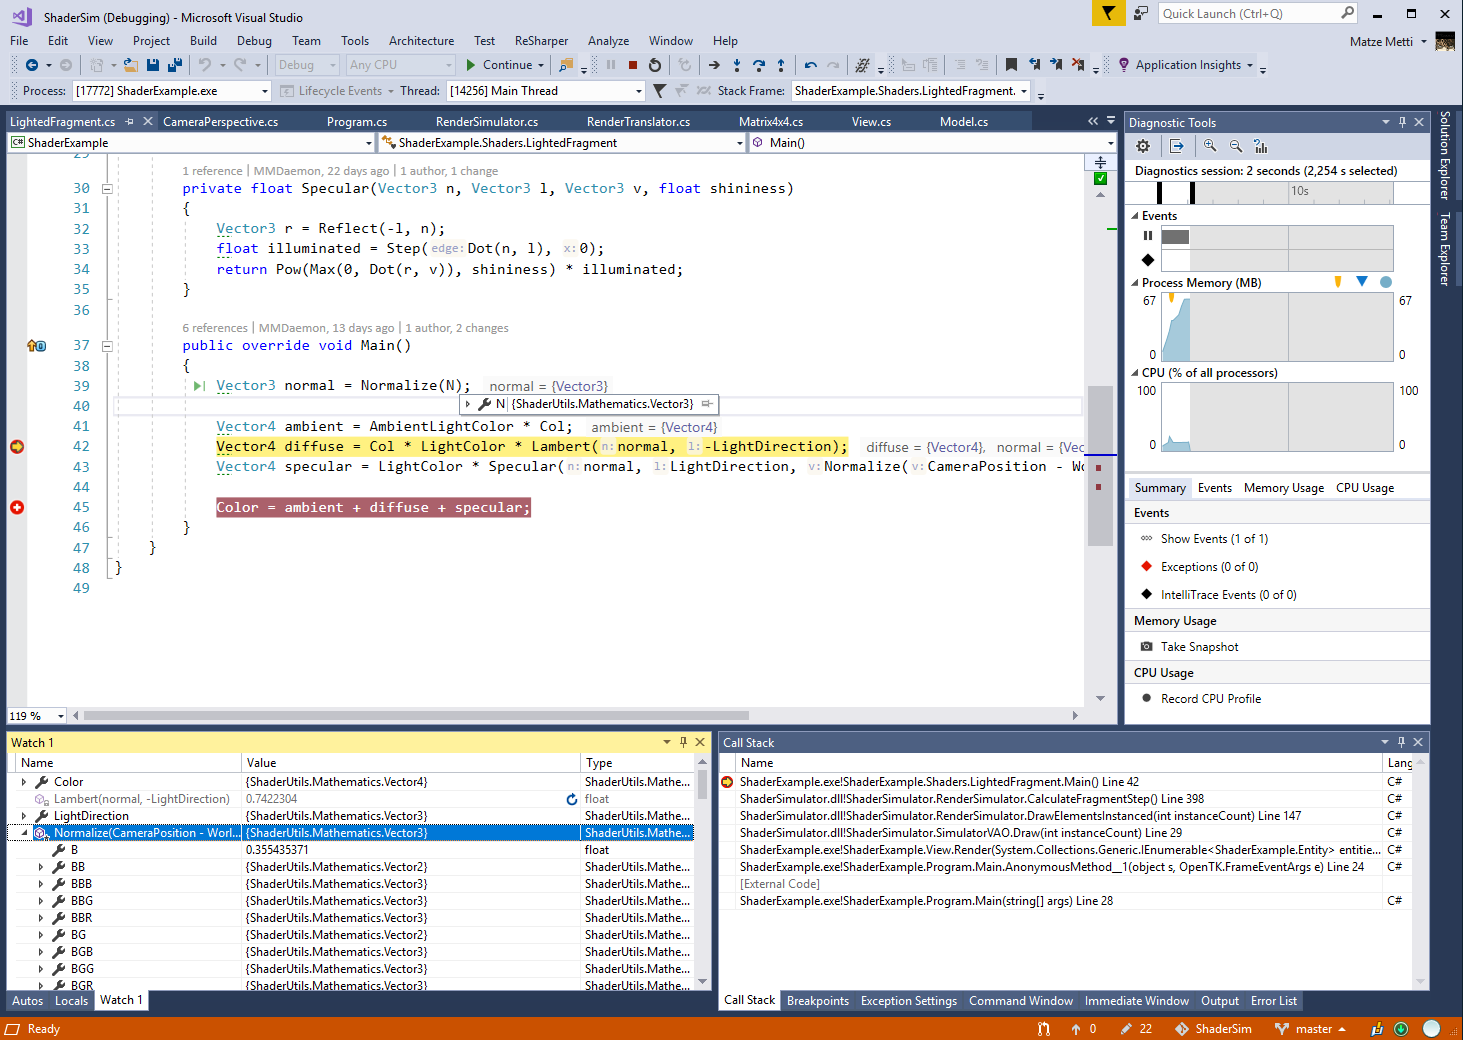
\includegraphics[angle=90,origin=c,scale=0.4]{debugging.png}
  \caption[Screenshot of debug screen within VisualStudio]{Debugging shader with different tools in VisualStudio: setting breakpoints, breakpoints with conditions, stepping through the code, variable inspection, navigating through the call stack}
  \label{fig:debugging}
\end{figure}

The project implemented as part of this research is limited in its functionality but it serves as proof for the practicability of the presented methods. It is a functioning method which could be refined and realized in a full tool supporting different source and output languages.



